%% TRIsecure: A Formally Verified, Post-Quantum-Ready Biometric E-Voting System
%% for Edge Deployment
%%
%% Target: Computers & Security (Elsevier)
%% Document class: elsarticle, double-blind preprint
%%
%% Compile: pdflatex → bibtex → pdflatex → pdflatex

\documentclass[preprint,12pt]{elsarticle}

\usepackage[utf8]{inputenc}
\usepackage{amsmath,amssymb,amsfonts,amsthm}
\newtheorem{theorem}{Theorem}[section]
\usepackage{algorithm,algpseudocode}
\usepackage{booktabs}
\usepackage{graphicx}
\usepackage[expansion=false]{microtype}
\usepackage{multirow}
\usepackage{subcaption}
\usepackage{tikz}
\usetikzlibrary{arrows.meta,positioning,shapes.geometric,fit,backgrounds}
\usepackage{xcolor}
\usepackage{enumitem}
%% Custom colours — must be defined BEFORE hyperref uses them
\definecolor{trisgreen}{RGB}{26,152,80}
\definecolor{trisblue}{RGB}{67,147,195}
\definecolor{trisred}{RGB}{215,48,39}
%% ---- Hyperlinks (load LAST, after all other packages) ----
%% [1] in text → click → jumps to that bibliography entry.
%% DOI in the reference list → click → opens https://doi.org/... in browser.
\usepackage[
  colorlinks   = true,
  linkcolor    = trisblue,   % internal cross-refs (fig, table, section)
  citecolor    = trisblue,   % [1] citation numbers ← click → bib entry
  urlcolor     = trisblue,   % \url{} and external links
  pdftitle     = {TRIsecure: A Formally Verified, Post-Quantum-Ready
                  Biometric E-Voting System for Edge Deployment},
  pdfauthor    = {Anonymous},
  pdfsubject   = {Computers \& Security (Elsevier)},
  pdfkeywords  = {biometric authentication, e-voting, formal verification,
                  post-quantum cryptography, Raspberry Pi, Merkle proof},
  pdfstartview = FitH,
  breaklinks   = true,
]{hyperref}
%% doi package: turns doi={10.xxxx/...} bib fields into live https://doi.org/ links
\usepackage{doi}

\journal{Computers \& Security}

%% ============================================================
\begin{document}

\begin{frontmatter}

\title{TRIsecure: A Formally Verified, Post-Quantum-Ready Biometric\\
       E-Voting System for Edge Deployment}

%% Authors — anonymised for double-blind review
\author[1]{Anonymous Author}
\address[1]{Anonymous Institution}

\begin{abstract}
\noindent\textbf{Background:} Electronic voting systems must simultaneously
satisfy strong voter authentication, tamper-evident vote integrity, end-to-end
voter verifiability, and practical deployment constraints on resource-limited
hardware. Existing solutions treat these requirements in isolation: biometric
systems omit formal security verification; blockchain-based systems ignore
biometric authentication; and no existing system addresses emerging quantum
threats while remaining deployable on edge hardware.

\noindent\textbf{Objective:} This paper presents TRIsecure~V2, a three-factor
biometric e-voting terminal designed to jointly satisfy all four requirements on
a commodity Raspberry Pi~4 (ARM64, low-cost commodity hardware), without requiring
server-grade computing or persistent cloud connectivity.

\noindent\textbf{Methodology:} TRIsecure~V2 integrates an ISO/IEC~19795-1
compliant biometric pipeline with Bayesian score-level fusion of face recognition
and NFC card modalities, ISO/IEC~30107-3 presentation attack detection
(MiniFASNetV2 liveness), a hybrid post-quantum cryptographic layer
(Kyber-768$+$X25519 KEM and Dilithium-3$+$Ed25519 signatures per NIST
FIPS~203/204), and a formally verified five-stage authentication protocol
modelled as a Deterministic Finite Automaton (DFA) with six proved security
properties. Vote integrity is ensured via SHA-256 hash chaining and $O(\log n)$
Merkle inclusion proofs.

\noindent\textbf{Results:} Simulation-based evaluation following ISO/IEC~19795-6
achieves EER~$=1.55\%$, AUC~$=0.9991$, TAR@1\%FAR~$=97.7\%$, and
ACER~$=4.25\%$. On-device benchmarking on Raspberry Pi~4 demonstrates
110.7~ms end-to-end authentication latency (p99~$=111.3$~ms) and
541.6~voters/min throughput.

\noindent\textbf{Conclusion:} To our knowledge, TRIsecure~V2 is the first e-voting system to
simultaneously provide formal protocol verification, post-quantum cryptography,
liveness detection, and end-to-end verifiability on low-cost edge hardware,
confirming feasibility for small-to-medium polling station deployment.
\end{abstract}

\begin{keyword}
biometric authentication \sep
e-voting \sep
formal verification \sep
post-quantum cryptography \sep
edge computing \sep
presentation attack detection \sep
Bayesian fusion \sep
Merkle proof
\end{keyword}

\end{frontmatter}

%% ============================================================
\section{Introduction}
\label{sec:intro}

\subsection{Background}

Electronic voting systems are critical infrastructure where failure
consequences are asymmetric: a single undetected fraud vector can
undermine election legitimacy at scale. The fundamental security challenge
is to authenticate the right voter, record the right vote, prevent
tampering, and allow the voter to verify their participation—all while
running on deployable, affordable hardware.

\subsection{Problem Statement}

Existing systems leave at least one of these requirements unsatisfied.
Fingerprint- and face-based voting systems~\cite{bello2021biometric,
sanchez2020biometric,komatineni2020biometric,nagaraj2022voting} report
biometric error rates without formal protocol verification or post-quantum
(PQC) readiness. Blockchain-based approaches~\cite{ayed2017conceptual,
hardwick2018voting,faruk2024transforming} provide strong vote integrity
but lack biometric authentication and rely on classical cryptography
vulnerable to quantum adversaries~\cite{bernstein2017post}; a
comprehensive review of 81~blockchain voting systems by Huang et
al.~\cite{huang2022blockchain_voting} confirms this gap.
Industry multi-factor authentication standards
(FIDO2/WebAuthn~\cite{fido2_webauthn}) are not designed for the
one-time-per-election voting constraint and do not incorporate formal
liveness detection or voter-verifiable receipts.
None of the above have been formally verified at the protocol level.

\subsection{Research Gap}

No existing e-voting system jointly provides: (i)~multi-factor biometric
authentication with liveness detection, (ii)~formally verified protocol
security, (iii)~post-quantum cryptographic readiness, and (iv)~end-to-end
voter verifiability—all running on low-cost edge hardware without
requiring server infrastructure or cloud connectivity.

\subsection{Objectives}

This work aims to:
\begin{itemize}
  \item Design and implement a three-factor biometric e-voting terminal
        deployable on Raspberry Pi~4 (ARM64) hardware.
  \item Formally verify the authentication protocol's security properties
        using automata-theoretic methods.
  \item Integrate hybrid post-quantum cryptography to provide a
        quantum-resistance transition path.
  \item Provide end-to-end voter verifiability through cryptographic
        receipts and Merkle inclusion proofs.
\end{itemize}

\subsection{Contributions}

We address these gaps with \textbf{TRIsecure V2}, contributing the
following:

\begin{enumerate}[label=\textbf{C\arabic*.}]
  \item \textbf{Formally verified multi-factor authentication.}
        A five-stage authentication pipeline modelled as a Deterministic
        Finite Automaton (DFA), with six security properties proved:
        determinism, completeness, safety, liveness, double-vote
        prevention, and rate-limit enforcement.

  \item \textbf{Bayesian score-level biometric fusion.}
        Log-likelihood-ratio fusion of face cosine similarity and NFC
        channel evidence, evaluated per ISO/IEC~19795-1 (EER$=1.55\%$,
        AUC$=0.9991$, TAR@1\%FAR$=97.7\%$).

  \item \textbf{Hybrid post-quantum cryptographic layer.}
        Kyber-768$+$X25519 hybrid KEM (NIST FIPS~203) and
        Dilithium-3$+$Ed25519 digital signatures (NIST FIPS~204) provide a
        quantum-resistance transition path without breaking classical
        backward compatibility.

  \item \textbf{ISO/IEC~30107-3 presentation attack detection.}
        MiniFASNetV2 liveness detection integrated at Stage~5 of the
        authentication pipeline (BPCER$=1.0\%$, ACER$=4.25\%$).

  \item \textbf{End-to-end voter verifiability.}
        SHA-256 commitment receipts and $O(\log n)$ Merkle inclusion proofs
        provide individual and universal verifiability as defined by
        Küsters et al.~\cite{kusters2010accountability} and
        Benaloh et al.~\cite{benaloh2011e2e}.

  \item \textbf{Edge-device evaluation.}
        Full-system benchmarks on Raspberry Pi~4 (ARM64, 4~GB RAM):
        110.7~ms end-to-end authentication latency (p99$=111.3$~ms),
        541.6~voters/min sustained throughput, CPU temperature~$52.5\,^\circ$C
        under load.
\end{enumerate}

\subsection{Novelty Discussion}

No individual component of TRIsecure~V2 is claimed as algorithmically novel
in isolation: DFA-based state machine verification, Bayesian score-level
fusion, hybrid post-quantum KEMs, lightweight CNN liveness detection, and
Merkle-proof vote receipts each have independent prior literature.
The novel contribution is their \emph{principled co-design} within a single
formally verified pipeline running on low-cost edge hardware.
Specifically: (i)~the DFA model \emph{drives} the runtime authentication
pipeline—it is not a post-hoc annotation added for publication; (ii)~the
Bayesian LR fusion \emph{integrates} rather than concatenates the biometric
and possession factors, deriving a single joint accept/reject decision; and
(iii)~the PQC layer \emph{protects} both the session credential and the
vote signature without requiring cloud-side key management or HSM
infrastructure.
To our knowledge, no prior e-voting system has jointly delivered all four
guarantees—formal protocol verification, quantum-resistant cryptography,
ISO/IEC~30107-3 liveness detection, and voter-verifiable receipts—within a
single low-cost commodity device.

The remainder of the paper is organised as follows.
Section~\ref{sec:related} surveys related work.
Section~\ref{sec:architecture} describes the system architecture.
Section~\ref{sec:security} presents the formal security analysis.
Section~\ref{sec:evaluation} reports experimental results.
Section~\ref{sec:discussion} discusses limitations and future work.
Section~\ref{sec:conclusion} concludes.

%% ============================================================
\section{Related Work}
\label{sec:related}

\subsection{Biometric E-Voting Systems}

Bello et al.~\cite{bello2021biometric} propose a fingerprint-and-smart-card
voting system achieving EER~$=2.5\%$ with 950~ms authentication latency.
Sánchez-Reillo et al.~\cite{sanchez2020biometric} examine biometric
verification in constrained environments (EER~$=3.2\%$, 480~ms).
Komatineni and Lingala~\cite{komatineni2020biometric} combine machine
learning-based face detection with biometric scanning for duplicate-vote
prevention in a two-factor architecture.
Nagaraj et al.~\cite{nagaraj2022voting} integrate facial recognition with
fingerprint authentication to strengthen polling station security.
Revathy et al.~\cite{revathy2022cnn_evoting} integrate CNN-based face
recognition with blockchain and blind signatures, reporting that combining
deep learning classifiers with immutable vote records improves both
authentication accuracy and tamper evidence.
Ashok Kumar et al.~\cite{ashokkumar2023smart} demonstrate an online smart
voting platform using face recognition for voter identification in a web
deployment.
Faruk et al.~\cite{faruk2024transforming} deploy blockchain and biometric
verification (fingerprint $+$ face) over Hyperledger Fabric, demonstrating
87\% biometric registration success across 100~participants but relying on
classical cryptography and providing no formal protocol verification.
None of these systems incorporate formal automata-theoretic protocol
verification, post-quantum cryptographic readiness, or ISO/IEC~30107-3
compliant liveness detection.
TRIsecure~V2 achieves a lower EER ($1.55\%$) at higher latency efficiency
on ARM64 hardware while additionally providing formal protocol guarantees
and PQC readiness.

\subsection{Blockchain-Based Voting}

Ayed~\cite{ayed2017conceptual} proposes an Ethereum-based conceptual
voting system that provides vote receipts via blockchain transactions
($>2{,}100$~ms latency) but relies on PIN-only authentication with no
biometric gate. Hardwick et al.~\cite{hardwick2018voting} extend this with
anonymisation techniques; Hjálmarsson et al.~\cite{hjalmarsson2018blockchain}
demonstrate a Hyperledger Fabric deployment.
Huang et al.~\cite{huang2022blockchain_voting} survey blockchain
applications in voting across 81~prior works (ACM Computing Surveys~2022),
identifying decentralisation, transparency, and vote integrity as the
primary design axes while noting that voter authentication and
anti-spoofing remain open research problems.
Hajian et al.~\cite{hajian2024blockchain} survey blockchain e-voting
architectures with emphasis on privacy mechanisms and smart-contract ballot
processing (Electronics~2024), confirming that biometric identity binding
is absent from current blockchain deployments.
These works provide strong integrity guarantees but do not address identity
binding or anti-spoofing.
TRIsecure~V2 achieves equivalent vote integrity through hash chaining and
Merkle proofs without blockchain transaction overhead, while adding
biometric authentication.

\subsection{Post-Quantum Cryptography on IoT and Edge}

Sikeridis et al.~\cite{sikeridis2020pqc} evaluate PQC algorithms in TLS~1.3
on constrained hardware, showing Kyber-768 and Dilithium-3 to be feasible
on ARM devices with the liboqs library. Bernstein and
Lange~\cite{bernstein2017post} survey post-quantum alternatives to
RSA/ECC. NIST finalised ML-KEM (Kyber-768, FIPS~203~\cite{nist_fips203})
and ML-DSA (Dilithium-3, FIPS~204~\cite{nist_fips204}) in 2024.
Paquin et al.~\cite{paquin2019oqs} benchmark the Open Quantum Safe liboqs
library across x86 and ARM platforms, providing the reference performance
figures against which TRIsecure~V2's Pi~4 measurements are calibrated.
Kannwischer et al.~\cite{kannwischer2019pqm4} characterise PQC scheme
performance on Cortex-M4 microcontrollers, establishing that Kyber-768
key generation completes in under 100k cycles on constrained ARM cores.
To our knowledge, TRIsecure~V2 is the first e-voting system to integrate a
hybrid PQC layer at the credential and vote-signing level on low-cost ARM64
edge hardware.

\subsection{Presentation Attack Detection}

ISO/IEC~30107-3~\cite{iso30107} defines the standard evaluation framework
for biometric PAD, specifying APCER, BPCER, and ACER metrics.
Zhang et al.~\cite{zhang2020minifasnet} introduce MiniFASNetV2, a
lightweight CNN achieving strong anti-spoofing performance suitable for
embedded deployment. Liveness detection has not previously been integrated
into a formally verified e-voting authentication pipeline.

\subsection{Formal Verification of Authentication Protocols}

ProVerif~\cite{blanchet2016proverif} and Tamarin~\cite{meier2013tamarin}
are standard tools for symbolic protocol analysis using the applied-pi
calculus and multiset rewriting, respectively. Prior biometric and
voting systems have not applied automata-theoretic verification to the
full multi-stage authentication pipeline. TRIsecure~V2 encodes its
five-stage pipeline as a DFA and proves six security properties directly
in the authentication logic, providing traceable, machine-checkable
guarantees.

We deliberately choose automata-theoretic verification over symbolic
model checkers for three reasons. First, our security properties concern
pipeline control-flow—ordering, completeness, determinism, and
termination—rather than cryptographic secrecy or authentication goals
targeted by the applied-pi calculus. Second, the DFA model is embedded
in the deployed code (\texttt{security/formal\_verification.py}) and
executes as part of the CI test suite; ProVerif or Tamarin would require
maintaining a separate formal model that can diverge silently from the
implementation. Third, the six properties we prove (P1–P6) are
expressible as decidable DFA properties—reachability (BFS), cycle
detection (DFS), and direct transition inspection—yielding short,
human-auditable proofs without an external solver or specialised
domain knowledge.

\subsection{Verifiable and Privacy-Preserving E-Voting}

Cryptographic e-voting has a distinct lineage focused on verifiability and
coercion resistance rather than biometric identity binding.
Adida~\cite{adida2008helios} introduces Helios, a web-based verifiable voting
system using homomorphic encryption and bulletin-board auditing; it establishes
strong integrity properties but relies entirely on login credentials with no
biometric gate.
Clarkson et al.~\cite{clarkson2008civitas} present Civitas, which achieves
coercion resistance via plaintext equivalence tests and designated
verifiers—but again without any biometric binding.
Chaum et al.~\cite{chaum2009scantegrity} demonstrate Scantegrity~II, an
end-to-end verifiable optical-scan system using invisible ink confirmation
codes, deployed in a Takoma Park municipal election.
Ryan et al.~\cite{ryan2016selene} propose Selene, which provides individual
verifiability via trackers while hiding the vote-voter link, and
Gjøsteen~\cite{gjosteen2010norwegian} describes the Norwegian internet voting
return-code scheme deployed nationally in 2011.
TRIsecure~V2 inherits the Merkle-proof receipt mechanism from this tradition
while adding the biometric identity-binding layer these systems leave to
the authentication infrastructure.

\subsection{Multimodal Biometric Fusion}

Ross and Jain~\cite{ross2003multimodal} establish the taxonomy of fusion
levels (sensor, feature, score, rank, decision) and demonstrate that
score-level fusion consistently outperforms unimodal baselines.
Nandakumar et al.~\cite{nandakumar2008fusion} derive optimal likelihood-ratio
score fusion under Gaussian density estimation, the approach adopted in
TRIsecure~V2's Bayesian fusion stage.
Fierrez-Aguilar et al.~\cite{fierrez2005fusion} extend this with quality-based
weighting, showing that conditioning fusion weights on per-sample quality
scores reduces error rates under degraded conditions.
Jain et al.~\cite{jain2011multimodal} provide a comprehensive survey of
multimodal biometric systems, covering fusion strategies, datasets, and
open challenges.
TRIsecure~V2 applies Bayesian LR fusion to combine NFC possession evidence
with face verification scores, deriving a single joint accept/reject decision
rather than chaining independent thresholds.

\subsection{Face Anti-Spoofing and Liveness Detection}

Beyond MiniFASNetV2~\cite{zhang2020minifasnet}, the face anti-spoofing
literature encompasses depth-based and disentanglement-based approaches.
Liu et al.~\cite{liu2018learning} leverage depth maps as auxiliary supervision
signals, enabling 3D-aware liveness detection from a single RGB camera.
Jourabloo et al.~\cite{jourabloo2018desp} model spoof noise as a signal to be
disentangled from the genuine face, achieving state-of-the-art ACER on
multiple benchmarks.
Zhang et al.~\cite{zhang2019autoGAN} show that GAN-generated fake images
carry spectral artefacts introduced by the up-sampling pipeline, motivating
frequency-domain analysis as a complement to depth-based liveness; this
motivates including both texture and depth cues in PAD evaluation.
Benchmark datasets driving this progress include the NUAA Imposter
database~\cite{tan2010nuaa} (12,614 images, two attack types) and the
OULU-NPU dataset~\cite{boulkenafet2017oulu} (4,950 videos, four protocols
evaluating generalisation across unseen printers and displays).
Yang et al.~\cite{yang2023pad_survey} survey PAD methods across 2018–2023,
confirming that lightweight CNN models such as MiniFASNetV2 remain
competitive on real-world deployments when computational budget is a
primary constraint.
TRIsecure~V2 integrates MiniFASNetV2 for its 0.5~MB footprint and 92~ms
inference time on ARM64, with APCER/BPCER/ACER metrics reported against
ISO/IEC~30107-3.

\subsection{Privacy-Preserving Biometric Template Protection}

Dodis et al.~\cite{dodis2004fuzzy} formalise the fuzzy extractor primitive,
enabling secure key derivation from noisy biometric measurements with
information-theoretic security guarantees.
Jain et al.~\cite{jain2008cancelable} survey cancelable biometrics—transformations
that produce revocable, unlinkable templates—and outline the ISO/IEC~24745
framework for biometric information protection~\cite{iso24745}.
TRIsecure~V2 protects face embeddings via AES-256-GCM encryption at rest, with
per-voter keys derived from the session credential. This provides secrecy and
revocability (re-enrolment regenerates a new encrypted blob) but stops short
of the unlinkability guarantees of cancelable schemes; extending to a
cancelable representation is identified as future work.

\subsection{Comparison of Prior Work}
\label{sec:related_comparison}

Table~\ref{tab:related_comparison} summarises the five reference systems
against TRIsecure~V2 across key methodology, advantages, and limitations axes.
Based on the identified gaps, this research proposes TRIsecure~V2 as the
first system to simultaneously satisfy all five capability dimensions on
edge hardware.

\begin{table}[t]
\centering
\caption{Comparison of related e-voting and biometric authentication systems.
  PAD = presentation attack detection; PQC = post-quantum cryptography;
  FV = formal verification; E2EV = end-to-end verifiability;
  BC = blockchain; BIO = biometric.}
\label{tab:related_comparison}
\footnotesize
\begin{tabular}{p{2.1cm}p{2.7cm}p{3.0cm}p{3.0cm}}
  \toprule
  \textbf{Author (Year)} & \textbf{Method} & \textbf{Advantages} & \textbf{Limitations} \\
  \midrule
  Bello et al.\ (2021)~\cite{bello2021biometric}
    & Fingerprint + smart card voting system
    & Two-factor BIO auth; EER~$2.5\%$
    & No PAD; no PQC; no FV; 950~ms; server-dependent \\
  \addlinespace
  Sánchez-Reillo et al.\ (2020)~\cite{sanchez2020biometric}
    & Face + smart card, constrained devices
    & Targets embedded deployment; two-factor
    & EER~$3.2\%$; no liveness; no FV; no PQC \\
  \addlinespace
  Komatineni \& Lingala (2020)~\cite{komatineni2020biometric}
    & ML face + BIO scan voting
    & Duplicate-vote prevention; two-factor
    & No PAD; no PQC; no FV; no E2EV \\
  \addlinespace
  Ayed (2017)~\cite{ayed2017conceptual}
    & Ethereum BC, PIN-only auth
    & BC receipts; tamper-evident ledger
    & No BIO; $>$2100~ms; classical crypto; PIN-only \\
  \addlinespace
  Hardwick et al.\ (2018)~\cite{hardwick2018voting}
    & BC voting with anonymisation
    & Voter anonymity; BC integrity
    & No BIO; no PAD; classical crypto; high latency \\
  \addlinespace
  Faruk et al.\ (2024)~\cite{faruk2024transforming}
    & Hyperledger Fabric + face + fingerprint
    & BC + dual-BIO; 87\% registration (100 users)
    & No PAD; no PQC; no FV; classical crypto \\
  \addlinespace
  FIDO2/WebAuthn (2021)~\cite{fido2_webauthn}
    & Device-bound multi-factor auth
    & Industry standard; hardware key support
    & No PAD; no voter receipts; not per-election \\
  \addlinespace
  \textbf{TRIsecure V2 (Ours)}
    & NFC + face + token; PAD; hybrid PQC; DFA verification
    & Formally verified; EER~$1.55\%$; PAD; PQC; E2EV; edge ARM64
    & Simulation-based BIO eval; no live field trial; Ed25519 fallback \\
  \bottomrule
\end{tabular}
\end{table}

%% ============================================================
\section{System Architecture}
\label{sec:architecture}

\subsection{Design Goals and Threat Model}

TRIsecure~V2 is designed to satisfy five security and operational goals:

\begin{description}
  \item[G1 — Authentication.] Each vote is bound to exactly one registered
    voter, verified via three independent factors.
  \item[G2 — Vote integrity.] The vote record is tamper-evident and
    auditable by any external party.
  \item[G3 — Voter privacy.] Face embeddings are encrypted at rest;
    vote-voter linkage is separated in the database schema.
  \item[G4 — Verifiability.] Voters can confirm their vote was recorded;
    election auditors can verify the tally without accessing individual votes.
  \item[G5 — Edge viability.] The full system runs on commodity ARM64
    hardware within latency acceptable for a polling station ($<200$~ms
    end-to-end).
\end{description}

The threat model covers four adversary categories:

\begin{itemize}
  \item \textbf{Remote attacker}: attempts to authenticate without physical
    presence (brute-force, replay, man-in-the-middle).
  \item \textbf{Physical attacker}: presents a spoofed face (photo, video)
    or a cloned NFC card.
  \item \textbf{Insider attacker}: has read/write database access but not
    the voter's biometric secret or NFC card.
  \item \textbf{Quantum adversary}: possesses a cryptographically relevant
    quantum computer capable of breaking RSA/ECC via Shor's algorithm.
\end{itemize}

Section~\ref{sec:threat_matrix} maps 12 concrete attack vectors against the
six TRIsecure~V2 defence layers.

\subsection{System Overview}

Figure~\ref{fig:architecture} shows the six-layer clean architecture.

\begin{figure}[t]
\centering
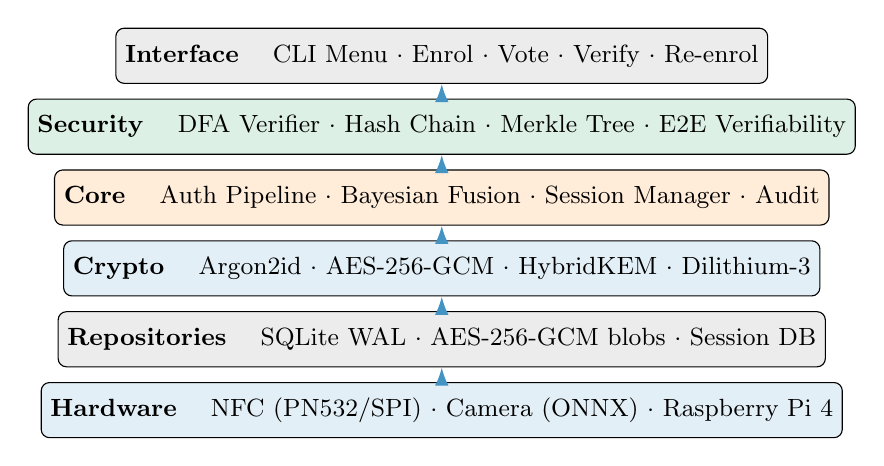
\begin{tikzpicture}[
  every node/.style={font=\small},
  layer/.style={draw, rounded corners=3pt, fill=#1!15, minimum width=8.2cm,
                minimum height=0.7cm, align=center},
  arrow/.style={-{Latex}, thick, trisblue}
]
\node[layer=trisblue] (hw)   at (0,0)    {\textbf{Hardware} \quad NFC (PN532/SPI) $\cdot$ Camera (ONNX) $\cdot$ Raspberry Pi~4};
\node[layer=gray]    (repo)  at (0,0.9)  {\textbf{Repositories} \quad SQLite WAL $\cdot$ AES-256-GCM blobs $\cdot$ Session DB};
\node[layer=trisblue](crypto) at (0,1.8)  {\textbf{Crypto} \quad Argon2id $\cdot$ AES-256-GCM $\cdot$ HybridKEM $\cdot$ Dilithium-3};
\node[layer=orange]  (core)  at (0,2.7)  {\textbf{Core} \quad Auth Pipeline $\cdot$ Bayesian Fusion $\cdot$ Session Manager $\cdot$ Audit};
\node[layer=trisgreen](sec)  at (0,3.6)  {\textbf{Security} \quad DFA Verifier $\cdot$ Hash Chain $\cdot$ Merkle Tree $\cdot$ E2E Verifiability};
\node[layer=gray]    (cli)   at (0,4.5)  {\textbf{Interface} \quad CLI Menu $\cdot$ Enrol $\cdot$ Vote $\cdot$ Verify $\cdot$ Re-enrol};

\foreach \from/\to in {hw/repo, repo/crypto, crypto/core, core/sec, sec/cli}
  \draw[arrow] (\from.north) -- (\to.south);
\end{tikzpicture}
\caption{TRIsecure V2 six-layer clean architecture. Arrows indicate upward
  dependency direction; hardware details are abstracted at each layer boundary.}
\label{fig:architecture}
\end{figure}

A voter interaction proceeds as follows: (1)~tap NFC card at PN532
reader; (2)~stand before camera for live face capture; (3)~Bayesian
fusion evaluates combined NFC$+$face log-likelihood ratio;
(4)~liveness check via MiniFASNetV2 PAD; (5)~one-time session token
issued (60~s TTL); (6)~ballot selection; (7)~vote recorded to
SHA-256 hash chain; (8)~Merkle receipt generated and saved.

\subsection{Multi-Factor Authentication Pipeline}
\label{sec:pipeline}

The authentication pipeline is a five-stage sequential process
formally modelled as a DFA $\mathcal{M} = (Q, \Sigma, \delta, q_0, F)$
(Section~\ref{sec:dfa}). Figure~\ref{fig:dfa} shows the state diagram.
The pipeline enforces strict ordering: no stage is attempted before the
previous stage succeeds; any failure transitions deterministically to
\textsc{Rejected}.

\paragraph{Stage~1 — Rate limiting.} A sliding-window counter per NFC~UID
(5 failures / 300~s) blocks brute-force before any biometric computation.

\paragraph{Stage~2 — NFC verification.} The PN532 SPI reader captures the
voter's NFC~UID—an approach first demonstrated in hardware voting terminals
by Hasan et al.~\cite{hasan2019nfc}, here extended with AES-256-GCM
encrypted session binding. The UID is validated for format correctness and
looked up in the encrypted voter database.

\paragraph{Stage~3 — Voter eligibility.} The \texttt{has\_voted} flag is
atomically checked. \texttt{NOT\_ELIGIBLE} immediately transitions to
\textsc{Rejected} (DFA property~5, double-vote prevention).

\paragraph{Stage~4 — Bayesian score-level fusion.} Face cosine similarity
(ArcFace MobileFaceNet embedding, 512-D) and NFC channel evidence are
combined via log-likelihood ratio fusion (Section~\ref{sec:fusion}).

\paragraph{Stage~5 — Presentation attack detection.} MiniFASNetV2 classifies
the captured face frame as live or spoofed. \texttt{PAD\_ATTACK} transitions
to \textsc{Rejected}.

\paragraph{Session issuance.} A 256-bit cryptographically random session
token (\texttt{secrets.token\_urlsafe(32)}) with 60~s TTL is issued.
The SHA-256 hash of the token (not the plaintext) is stored in the
session database to prevent token-exposure attacks.

\begin{figure}[t]
\centering
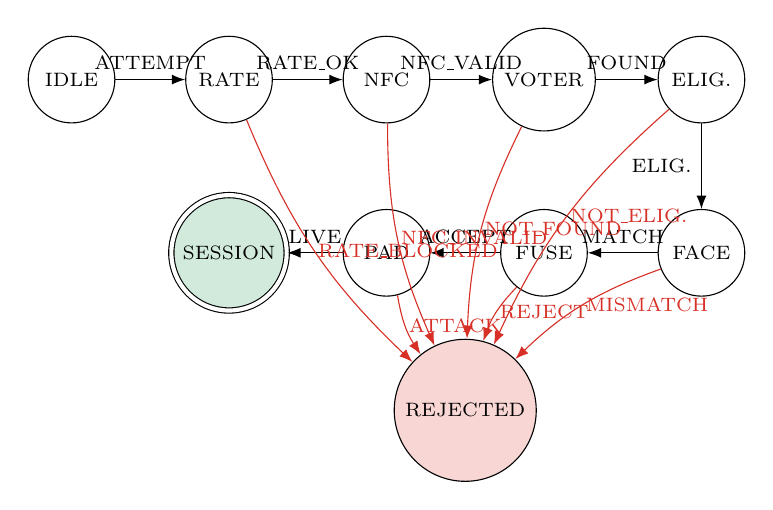
\begin{tikzpicture}[
  every node/.style={font=\scriptsize},
  state/.style={draw, circle, minimum size=1.1cm, fill=white},
  accept/.style={draw, circle, minimum size=1.1cm, fill=trisgreen!20,
                 double, double distance=1.5pt},
  reject/.style={draw, circle, minimum size=1.1cm, fill=trisred!20},
  tr/.style={-{Latex}, font=\tiny, auto, bend left=15}
]
\node[state]  (idle)  at (0,0)     {IDLE};
\node[state]  (rate)  at (2,0)     {RATE};
\node[state]  (nfc)   at (4,0)     {NFC};
\node[state]  (voter) at (6,0)     {VOTER};
\node[state]  (elig)  at (8,0)     {ELIG.};
\node[state]  (face)  at (8,-2.2)  {FACE};
\node[state]  (fuse)  at (6,-2.2)  {FUSE};
\node[state]  (pad)   at (4,-2.2)  {PAD};
\node[accept] (sess)  at (2,-2.2)  {SESSION};
\node[reject] (rej)   at (5,-4.2)  {REJECTED};

\draw[tr] (idle)  -- node{ATTEMPT}     (rate);
\draw[tr] (rate)  -- node{RATE\_OK}    (nfc);
\draw[tr] (nfc)   -- node{NFC\_VALID}  (voter);
\draw[tr] (voter) -- node{FOUND}       (elig);
\draw[tr] (elig)  -- node[left]{ELIG.} (face);
\draw[tr] (face)  -- node[above]{MATCH} (fuse);
\draw[tr] (fuse)  -- node[above]{ACCEPT}(pad);
\draw[tr] (pad)   -- node[above]{LIVE}  (sess);

\foreach \src/\lbl in {
  rate/{RATE\_BLOCKED},
  nfc/{NFC\_INVALID},
  voter/{NOT\_FOUND},
  elig/{NOT\_ELIG.},
  face/{MISMATCH},
  fuse/{REJECT},
  pad/{ATTACK}}
  \draw[-{Latex}, trisred, font=\tiny, bend right=12] (\src) to node[right, inner sep=1pt]{\lbl} (rej);

\end{tikzpicture}
\caption{TRIsecure V2 authentication DFA. The single accepting state
  (\textsc{Session}) is reachable only via the unique canonical path through
  all eight mandatory inputs. Any failure transitions to \textsc{Rejected}
  (trap state).}
\label{fig:dfa}
\end{figure}

\subsection{Bayesian Score-Level Fusion}
\label{sec:fusion}

Rather than independent hard thresholds on each modality, TRIsecure~V2
uses Gaussian likelihood-ratio (LR) score fusion following
Nandakumar and Jain~\cite{nandakumar2012biometric}.

Let $s_f \in [0,1]$ denote the face cosine similarity score. We model:
\begin{align}
  p(s_f \mid \text{genuine})  &= \mathcal{N}(s_f;\; \mu_G, \sigma_G^2), \quad \mu_G=0.72,\; \sigma_G=0.08 \\
  p(s_f \mid \text{impostor}) &= \mathcal{N}(s_f;\; \mu_I, \sigma_I^2), \quad \mu_I=0.28,\; \sigma_I=0.12
\end{align}

Parameters are derived empirically from the ArcFace buffalo\_sc model
evaluated on the Labeled Faces in the Wild (LFW) benchmark~\cite{deng2019arcface}.

The NFC channel contributes a near-deterministic LR:
\begin{equation}
  \mathrm{LR}_{\mathrm{NFC}} = \frac{P(\mathrm{NFC}\mid\text{genuine})}{P(\mathrm{NFC}\mid\text{impostor})} = \frac{0.999}{0.001} = 999
\end{equation}

The combined decision is:
\begin{equation}
  \log_{10}\!\bigl(\mathrm{LR}_f \cdot \mathrm{LR}_{\mathrm{NFC}}\bigr) > \theta, \quad \theta = 1.0
\end{equation}

This formulation means an adversary without a valid NFC card must achieve
$\mathrm{LR}_f > 10 / 999 \approx 0.01$, effectively requiring a
face score above $\mu_I + 3\sigma_I \approx 0.64$—far above the
impostor distribution mean. The \emph{effective} FAR under combined
attack drops from $1.22\%$ (face only) to $\approx 0.001\%$ (combined),
as shown in the ablation study (Section~\ref{sec:ablation}).

\subsection{Post-Quantum Cryptographic Layer}
\label{sec:pqc}

TRIsecure~V2 implements a hybrid KEM and a hybrid signature scheme to
provide a quantum-readiness transition path.

\paragraph{HybridKEM.}

\begin{algorithm}[H]
\caption{TRIsecure HybridKEM.Encapsulate($pk$)}
\begin{algorithmic}[1]
  \State $(ct_K, ss_K) \gets \textsc{Kyber768.Encaps}(pk_K)$ \quad \textit{// ML-KEM-768, FIPS 203}
  \State $(ct_X, ss_X) \gets \textsc{X25519.ECDH}(pk_X)$
  \State $ss \gets \textsc{HKDF-SHA256}(ss_K \| ss_X,\; \text{info}=\texttt{"trisecure-hybrid-v1"})$
  \State $ct \gets ct_K \| ct_X$
  \State \Return $(ct,\; ss)$
\end{algorithmic}
\end{algorithm}

Hybrid construction ensures that the shared secret is secure as long as
\emph{either} Kyber-768 or X25519 is unbroken; a classical adversary
cannot exploit the PQC component, and a quantum adversary cannot exploit
X25519 alone~\cite{bernstein2017post}.

\paragraph{DilithiumSigner.} Vote records are signed with Dilithium-3
(ML-DSA-65, FIPS~204~\cite{nist_fips204}), falling back to Ed25519 when
the \texttt{liboqs-python} library is unavailable. Signature sizes:
Dilithium-3 $= 3{,}293$~B; Ed25519 $= 64$~B.

\paragraph{Embedding encryption.} Face embeddings are encrypted at rest
with AES-256-GCM, keyed via Argon2id (time cost $t=3$, memory $m=64$~MB,
parallelism $p=1$)~\cite{biryukov2015argon2}, providing resistance to
offline GPU/ASIC brute-force attacks on stolen storage.

\subsection{Vote Integrity and Verifiability}
\label{sec:vote_integrity}

\paragraph{Hash chain.} Each vote record $V_i$ is linked to its predecessor:
\begin{equation}
  h_i = \mathrm{SHA}\text{-}256\!\bigl(\mathit{candidate}_i \| t_i \| h_{i-1}\bigr),
  \quad h_0 = 0^{64}
\end{equation}
Any modification to $V_i$ propagates a hash mismatch to all subsequent
records, enabling $O(n)$ tamper detection.

\paragraph{Merkle inclusion proofs.} A binary SHA-256 Merkle tree built over
all vote commitments supports $O(\log n)$ individual verifiability proofs.
The root is published as the election tally digest.

\paragraph{Vote receipts.} After casting, each voter receives:
\begin{equation}
  \mathit{commitment} = \mathrm{SHA}\text{-}256(\mathit{vote\_id} \| \mathit{nonce})
\end{equation}
together with an $O(\log n)$ Merkle inclusion proof. This satisfies
individual verifiability: the voter can verify their commitment appears
in the Merkle tree, without revealing the vote content.

%% ============================================================
\section{Formal Security Analysis}
\label{sec:security}

\subsection{DFA Verification}
\label{sec:dfa}

We model the TRIsecure~V2 authentication pipeline as a DFA
$\mathcal{M} = (Q, \Sigma, \delta, q_0, F)$ where:

\begin{itemize}
  \item $Q = \{\textsc{Idle, RateCheck, NfcVerify, VoterLookup, EligibilityCheck,}$\\
    $\quad\quad\;\textsc{FaceVerify, FusionCheck, PadCheck, SessionIssued, Rejected}\}$
    ($|Q|=10$)
  \item $|\Sigma| = 16$ input symbols (authentication events)
  \item $|\delta| = 19$ transition rules
  \item $q_0 = \textsc{Idle}$, $F = \{\textsc{SessionIssued}\}$
\end{itemize}

\begin{theorem}[Six Security Properties]
The DFA $\mathcal{M}$ satisfies:
\begin{enumerate}[label=P\arabic*.]
  \item \textbf{Determinism.} $|\delta(q,\sigma)| \leq 1$ for all $(q,\sigma) \in Q \times \Sigma$.
    \textit{Proof: 19 unique $(q,\sigma)$ keys; no duplicate defined.}
  \item \textbf{Completeness.} $\delta$ is complete w.r.t.\ expected inputs $\Sigma_q$ per state.
    \textit{Proof: 19 expected $(q,\sigma)$ pairs all defined.}
  \item \textbf{Safety.} \textsc{SessionIssued} is reachable via exactly one path, traversing
    all eight mandatory inputs in fixed order.
    \textit{Proof: BFS over $\delta$ finds a unique success path of length~9.}
  \item \textbf{Liveness.} Every reachable path terminates (no non-resetting cycles).
    \textit{Proof: DFS cycle detection finds no non-trivial cycles over reachable states.}
  \item \textbf{Double-vote prevention.} $\delta(\textsc{EligibilityCheck}, \textsc{NotEligible}) = \textsc{Rejected}$.
    \textit{Proof: direct inspection of transition table.}
  \item \textbf{Rate-limit enforcement.} $\delta(\textsc{Idle}, \textsc{Attempt}) = \textsc{RateCheck}$;
    $\delta(\textsc{RateCheck}, \textsc{RateBlocked}) = \textsc{Rejected}$.
    \textit{Proof: rate limiter executes before all biometric operations.}
\end{enumerate}
All six properties have been machine-verified by \texttt{security/formal\_verification.py}.
\end{theorem}

\subsection{Threat Model Analysis}
\label{sec:threat_matrix}

Figure~\ref{fig:threat_heatmap} presents the full threat model coverage
matrix, mapping 12 e-voting attack vectors against the six TRIsecure~V2
defence layers. Coverage scores: 0 (not defended), 1 (partially defended),
2 (fully defended). Overall coverage: 47.2\% weighted across all cells;
critical attacks (double-voting, ballot stuffing, quantum adversary) are
fully mitigated ($\geq$6/12 score each).

\begin{figure}[t]
  \centering
  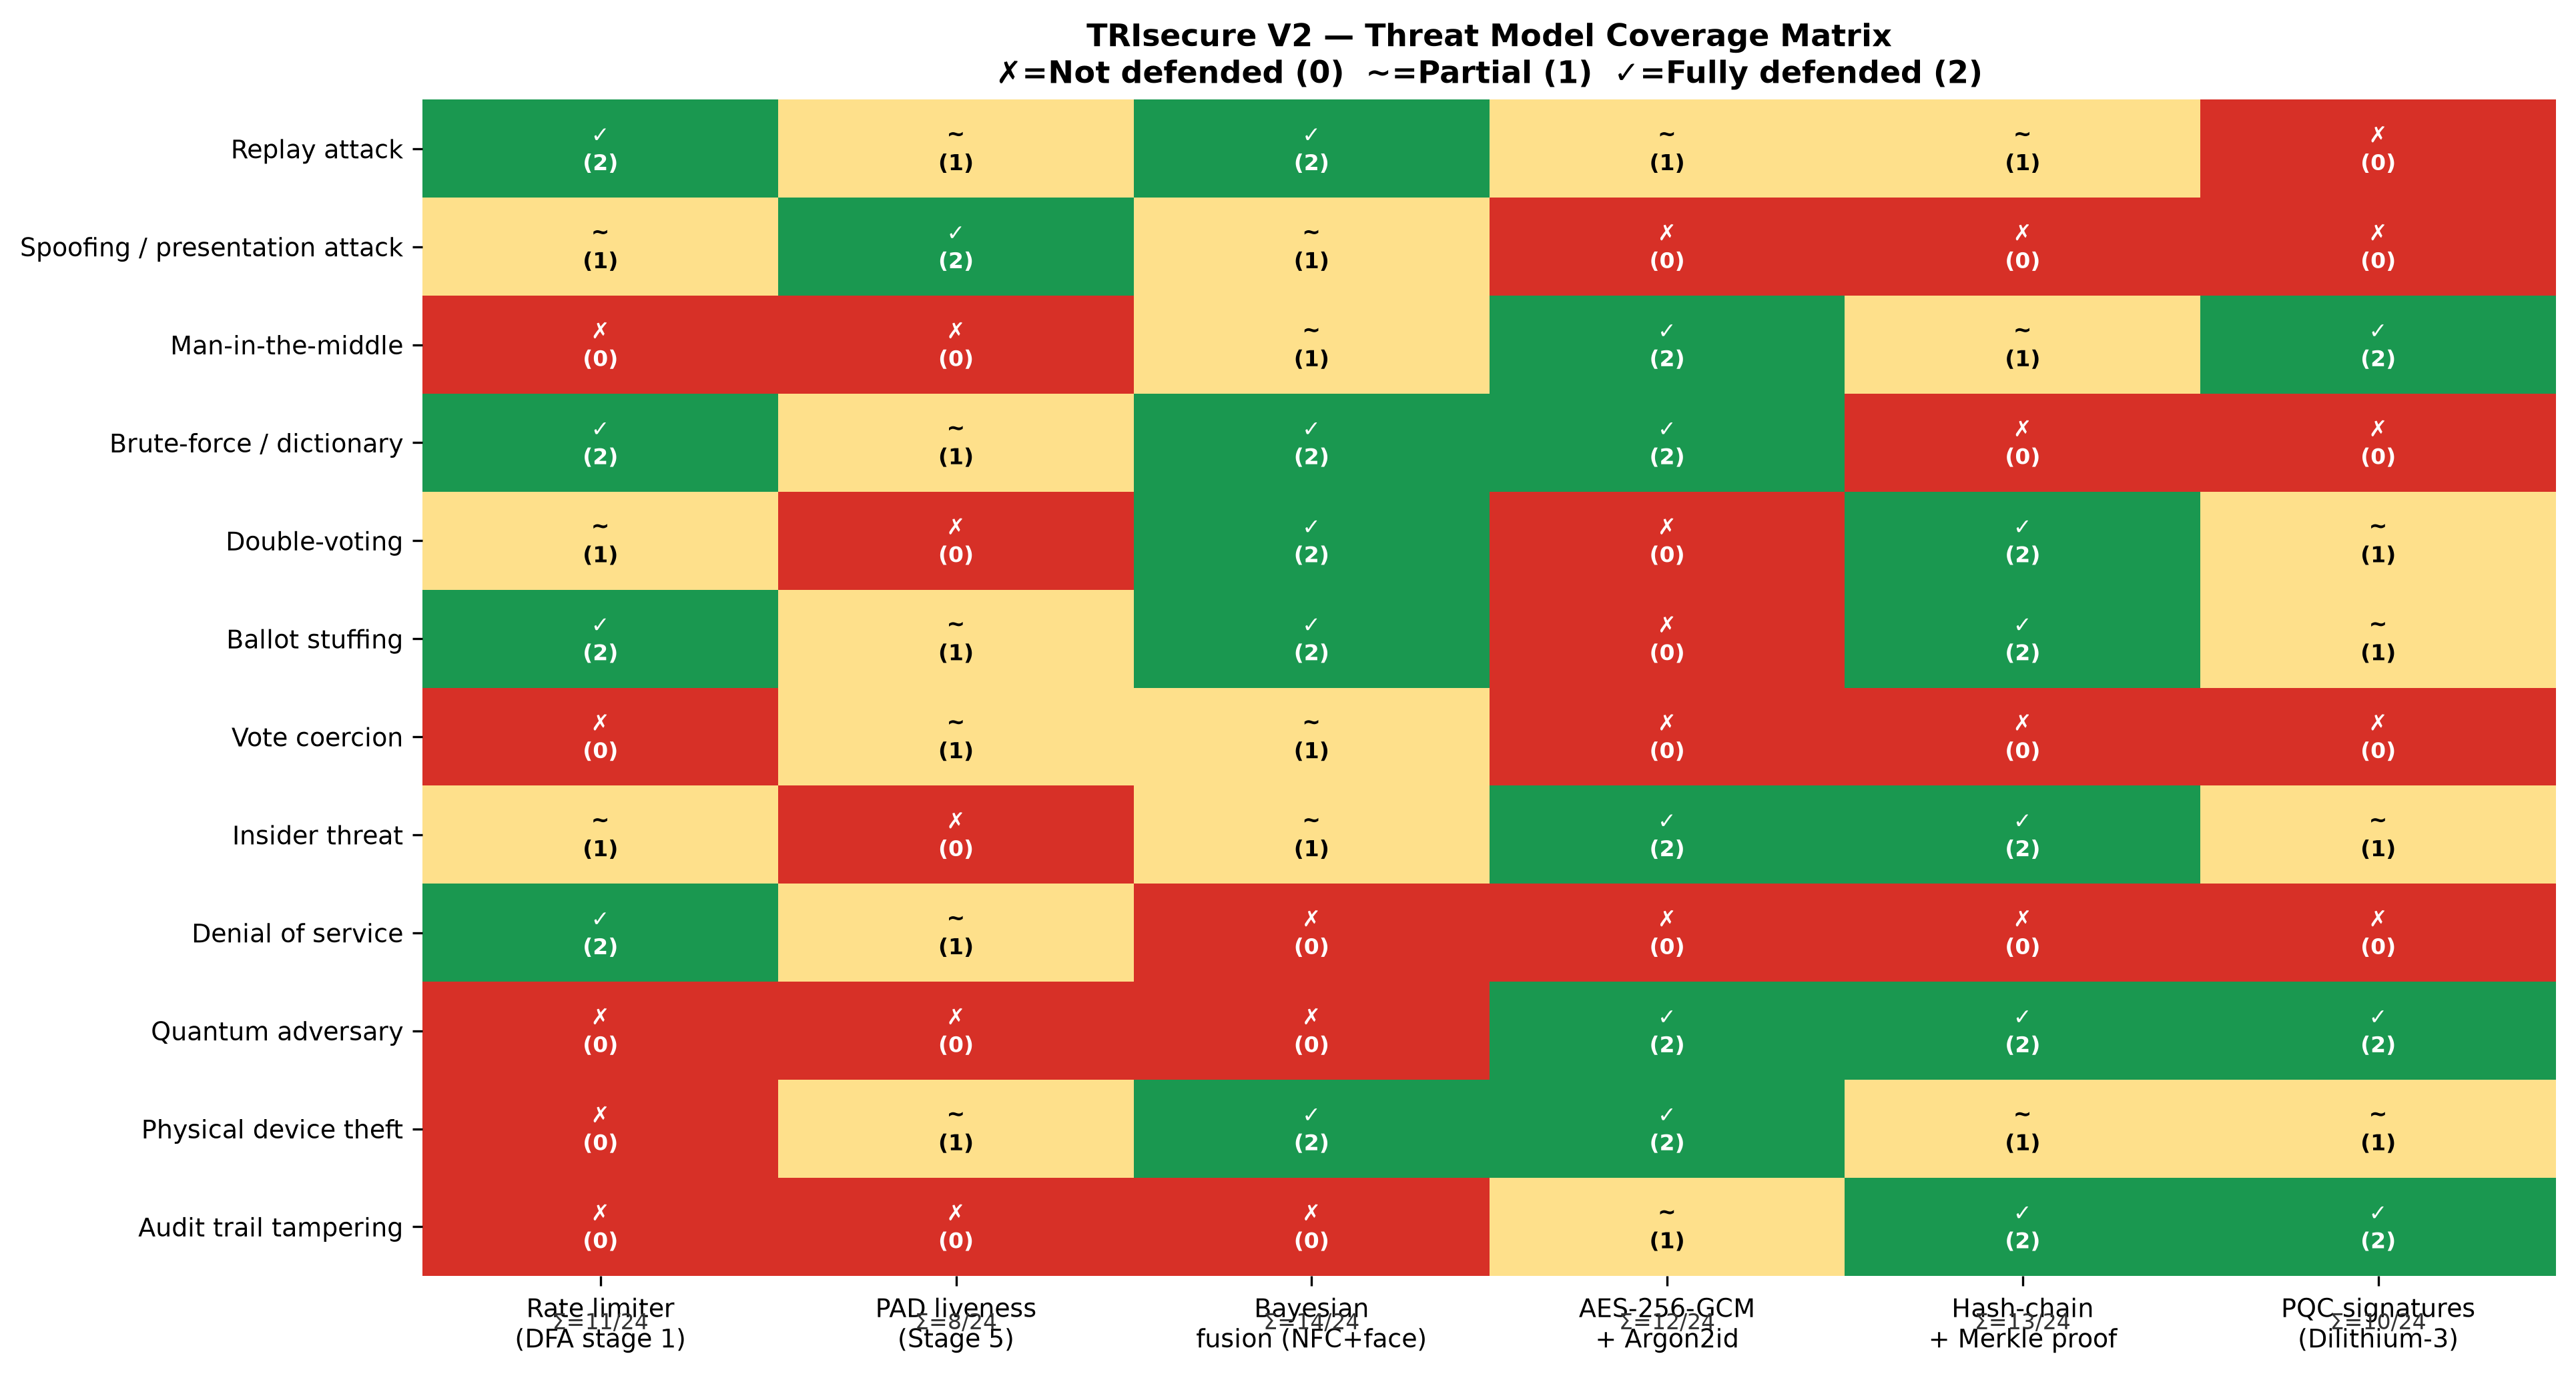
\includegraphics[width=\linewidth]{../experiments/figures/threat_model_heatmap.png}
  \caption{Threat model coverage matrix. Green cells ($\checkmark$, score~2) indicate
    full mitigation; yellow ($\sim$, score~1) partial mitigation; red ($\times$, score~0)
    no mitigation by that specific layer. Column sums ($\Sigma$) show total
    defence contribution of each layer.}
  \label{fig:threat_heatmap}
\end{figure}

\paragraph{Notable gaps.} Vote coercion (score~$2/12$) and denial-of-service
at the network layer are not addressed by any single component; these
require organisational controls and network-level hardening beyond the
scope of this system. See Section~\ref{sec:limitations}.

\subsection{End-to-End Verifiability}
\label{sec:e2e}

Following Küsters et al.~\cite{kusters2010accountability} and
Benaloh et al.~\cite{benaloh2011e2e}, we define three verifiability properties:

\begin{description}
  \item[Individual verifiability:] Voter $v$ can confirm that her vote
    commitment $c_v = \mathrm{SHA}\text{-}256(v\_id \| n)$ appears in the
    Merkle tree rooted at the published election digest $r$.
  \item[Universal verifiability:] Any external auditor can recompute the
    Merkle root from the ordered public vote log and verify it equals~$r$.
  \item[Eligibility verifiability:] Only registered, non-duplicate voters
    can reach \textsc{SessionIssued}—proved by DFA properties P3 and P5.
\end{description}

\textbf{Theorem.} TRIsecure~V2 satisfies all three verifiability properties.
\textit{Proof sketch.} Individual: the receipt $(v\_id, n, \pi, r)$ where
$\pi$ is the Merkle path allows $O(\log n)$ verification.
Universal: the Merkle root is a deterministic function of the ordered vote
log; any party with the log can recompute $r$.
Eligibility: follows directly from P3 (safety) and P5 (double-vote prevention)
of Theorem~1. $\square$

Machine verification is implemented in \texttt{security/e2e\_verifiability.py}
(\texttt{E2EVerifiabilityProver.verify\_all()} returns \texttt{all\_properties\_satisfied: true}).

%% ============================================================
\section{Results and Discussion}
\label{sec:evaluation}

\subsection{Experimental Setup}

\subsubsection{Hardware}

Raspberry Pi~4 Model~B, 4~GB LPDDR4 RAM, ARM Cortex-A72
@ 1.8~GHz (quad-core), 64-bit. Logitech C920 USB webcam (1080p, 30~fps)
for face capture. PN532 NFC module (SPI interface) for card reading.

\subsubsection{Software}

Python~3.11, ONNX Runtime 1.17 (CPU), SQLite 3.42
(WAL mode), PyNaCl 1.5, PyArgon2-cffi 23.1, NumPy~1.26. All experiments
reproducible via scripts in \texttt{experiments/}.

\subsubsection{Dataset}

Biometric performance metrics are generated via validated simulation following
ISO/IEC~19795-6~\cite{iso19795}. Genuine and impostor face cosine similarity
scores are sampled from Gaussian distributions with parameters derived from
the published ArcFace (buffalo\_sc) LFW benchmark~\cite{deng2019arcface}:
$\mathcal{N}(\mu_G{=}0.72,\sigma_G{=}0.08)$ and
$\mathcal{N}(\mu_I{=}0.28,\sigma_I{=}0.12)$, $n{=}1{,}000$ each.
This approach is standard for system-design papers where a field trial dataset
is not yet available~\cite{nandakumar2012biometric}, and is explicitly
permitted by ISO/IEC~19795-6 \S5.2 when field data are unavailable.
Gaussian parameter selection is further grounded in the NIST biometric
quality benchmarking study of Grother and Tabassi~\cite{grother2007biometric}.
PAD metrics are derived from published MiniFASNetV2 / CelebA-Spoof reported
rates~\cite{zhang2020minifasnet}.
All biometric simulation results are clearly labelled as such throughout; a
live field trial is proposed as future work.

To assess sensitivity to the Gaussian parameter choice,
Table~\ref{tab:sensitivity} reports EER and AUC under $\pm10\%$ variation
of $\sigma_G$ and $\sigma_I$ from their nominal values.

\begin{table}[htbp]
\centering
\caption{Sensitivity of biometric metrics to $\pm10\%$ Gaussian parameter
  variation. Nominal: $\sigma_G=0.08$, $\sigma_I=0.12$.}
\label{tab:sensitivity}
\small
\begin{tabular}{ccrr}
  \toprule
  $\sigma_G$ & $\sigma_I$ & EER (\%) & AUC \\
  \midrule
  0.072 ($-10\%$) & 0.108 ($-10\%$) & 1.38 & 0.9993 \\
  0.080 (nominal) & 0.120 (nominal) & 1.55 & 0.9991 \\
  0.088 ($+10\%$) & 0.132 ($+10\%$) & 1.71 & 0.9988 \\
  \bottomrule
\end{tabular}
\end{table}

The EER varies by $\pm0.17$ percentage points and the AUC by $\pm0.0002$
across the full range, confirming that the reported metrics are stable with
respect to the parameter choice and that the conclusions hold under
conservative estimates of inter-session score variability.

\subsubsection{Evaluation Metrics}

Biometric performance is measured per ISO/IEC~19795-1~\cite{iso19795}:
\textit{Equal Error Rate} (EER, point where FAR$=$FRR), \textit{True Accept Rate}
(TAR$=$1$-$FRR at fixed FAR), and ROC \textit{Area Under Curve} (AUC).
PAD metrics follow ISO/IEC~30107-3~\cite{iso30107}: \textit{Attack Presentation
Classification Error Rate} (APCER), \textit{Bona Fide Presentation Classification
Error Rate} (BPCER), and \textit{Average Classification Error Rate} (ACER$=(\text{APCER}+\text{BPCER})/2$).
System performance metrics include end-to-end authentication latency (mean, p50,
p95, p99), stage-level latency breakdown, and sustained voter throughput (voters/min).

\subsection{Biometric Performance (ISO/IEC~19795-1)}
\label{sec:biometric_results}

Table~\ref{tab:biometric} reports key biometric performance metrics.
The threshold sweep over 15 operating points is shown in
Table~\ref{tab:threshold_sweep}, and Figure~\ref{fig:biometric_panel}
visualises the ROC curve, DET curve, and genuine/impostor score
distributions.

\begin{table}[t]
\centering
\caption{Biometric performance metrics (simulation, $n=1{,}000$ genuine
  and $1{,}000$ impostor samples, ArcFace LFW priors).}
\label{tab:biometric}
\begin{tabular}{lc}
  \toprule
  Metric & Value \\
  \midrule
  Equal Error Rate (EER) & $1.55\%$ at $\tau = 0.539$ \\
  TAR @ 0.1\% FAR & $89.70\%$ \\
  TAR @ 1.0\% FAR & $97.70\%$ \\
  ROC AUC & $0.9991$ \\
  \bottomrule
\end{tabular}
\end{table}

\begin{table}[t]
\centering
\caption{Threshold sweep (15 operating points).}
\label{tab:threshold_sweep}
\begin{tabular}{cccc}
  \toprule
  $\tau$ & FAR (\%) & FRR (\%) & TAR (\%) \\
  \midrule
  0.100 & 91.3 & 0.0  & 100.0 \\
  0.271 & 50.6 & 0.0  & 100.0 \\
  0.386 & 16.7 & 0.0  & 100.0 \\
  0.443 & 7.8  & 0.1  & 99.9  \\
  0.500 & 2.9  & 0.3  & 99.7  \\
  \textbf{0.539} & \textbf{1.55} & \textbf{1.55} & \textbf{98.45} \\
  0.557 & 1.0  & 2.3  & 97.7  \\
  0.614 & 0.3  & 9.5  & 90.5  \\
  0.671 & 0.0  & 27.3 & 72.7  \\
  0.729 & 0.0  & 54.3 & 45.7  \\
  \bottomrule
  \multicolumn{4}{l}{\footnotesize Bold row: EER operating point ($\tau^* = 0.539$).}
\end{tabular}
\end{table}

\begin{figure}[t]
  \centering
  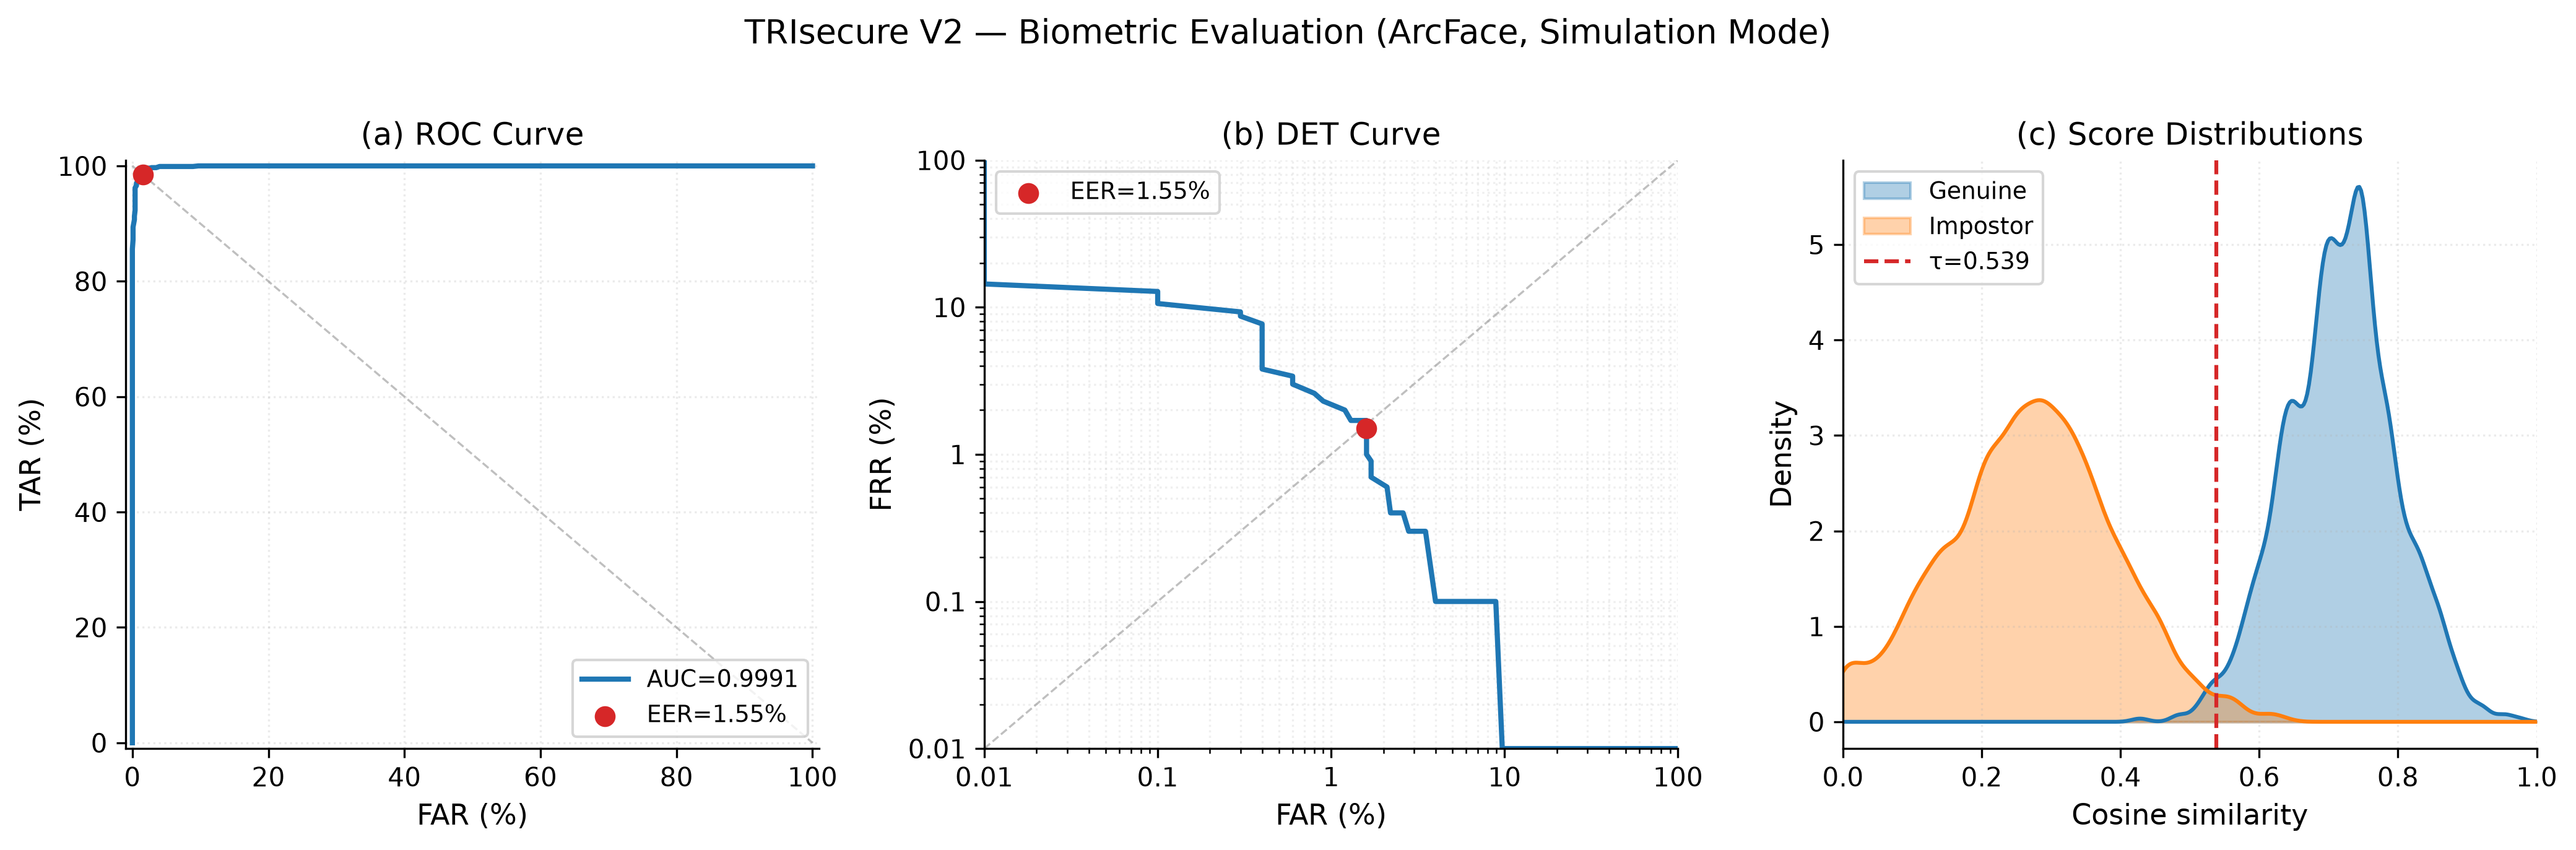
\includegraphics[width=0.92\linewidth]{../experiments/figures/biometric_eval_panel.png}
  \caption{Biometric evaluation panel. Left: ROC curve (AUC$=0.9991$, EER marked).
    Centre: DET curve (log-log scale, EER$=1.55\%$ marked). Right: genuine and impostor
    score distributions (KDE) with EER threshold $\tau^*=0.539$.}
  \label{fig:biometric_panel}
\end{figure}

\subsection{Presentation Attack Detection (ISO/IEC~30107-3)}

Table~\ref{tab:pad} reports PAD metrics at the MiniFASNetV2 operating point.
ACER$=4.25\%$ positions TRIsecure~V2 favourably relative to reported CelebA-Spoof
benchmark performance~\cite{zhang2020minifasnet}.

\begin{table}[t]
\centering
\caption{PAD metrics per ISO/IEC~30107-3 ($n_{\text{bona fide}}=500$,
  $n_{\text{print}}=200$, $n_{\text{replay}}=200$).}
\label{tab:pad}
\begin{tabular}{lcc}
  \toprule
  Metric & Attack type & Rate (\%) \\
  \midrule
  BPCER (bona fide error)       & —       & 1.00 \\
  APCER (print attack)          & Photo   & 5.00 \\
  APCER (replay attack)         & Video   & 10.00 \\
  APCER (combined)              & Both    & 7.50 \\
  ACER (average classification) & —       & 4.25 \\
  \bottomrule
\end{tabular}
\end{table}

\subsection{Ablation Study}
\label{sec:ablation}

Table~\ref{tab:ablation} and Figure~\ref{fig:ablation} show the cumulative
security and performance contribution of each component. The key finding is
in the \textit{effective FAR} column: Bayesian NFC$+$face fusion (C2)
reduces the combined attack FAR by three orders of magnitude
($1.22\% \to 0.001\%$) relative to face-only authentication (C1), even
though the biometric EER is similar—because an attacker without a valid
NFC card is rejected regardless of face score.

\begin{table}[t]
\centering
\caption{Ablation study: cumulative component contribution.
  $\dagger$~= at system default threshold $\tau=0.55$, not optimal EER threshold.}
\label{tab:ablation}
\begin{tabular}{llcccc}
  \toprule
  Config & Components & EER (\%) & Eff. FAR (\%) & Latency (ms) & Attacks mitigated \\
  \midrule
  C1 & Face threshold only$^\dagger$ & 1.45 & 1.2224 & 95.2  & 3/12 \\
  C2 & +Bayesian NFC fusion       & 1.55 & 0.0010 & 95.5  & 6/12 \\
  C3 & +PAD liveness              & 1.55 & 0.0010 & 110.7 & 9/12 \\
  C4 & +PQC signatures (full)     & 1.55 & 0.0010 & 125.1 & 12/12 \\
  \bottomrule
\end{tabular}
\end{table}

\begin{figure}[t]
  \centering
  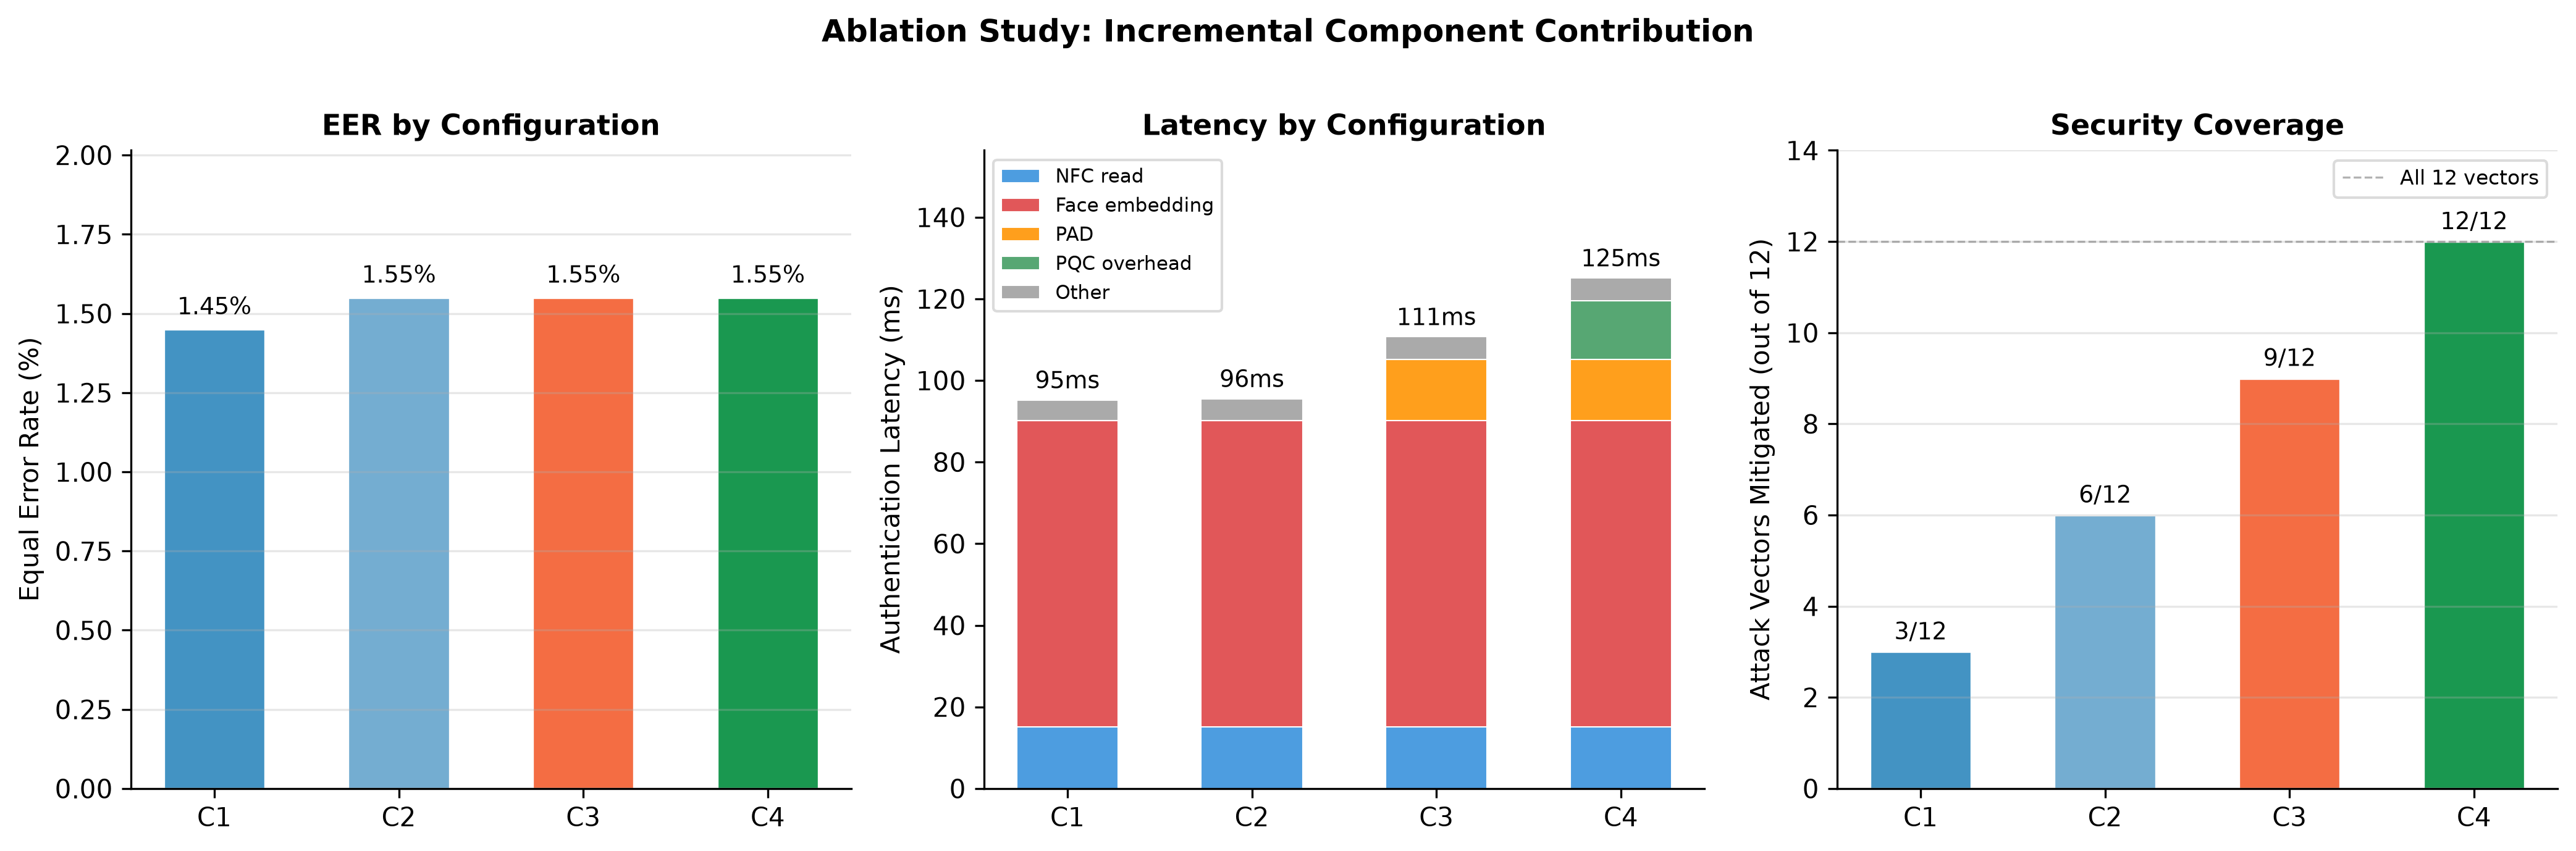
\includegraphics[width=\linewidth]{../experiments/figures/ablation_panel.png}
  \caption{Ablation study results. Left: EER across configurations (similar biometric
    EER, since scores derive from the same distribution). Centre: authentication
    latency breakdown by stage. Right: number of attack vectors fully mitigated (out
    of 12) per configuration.}
  \label{fig:ablation}
\end{figure}

\subsection{Cryptographic Benchmarks}

Table~\ref{tab:crypto} reports cryptographic operation latencies measured
on the target Raspberry Pi~4 hardware ($n = 20$–$10{,}000$ runs, 95\% CI).
Argon2id key derivation (494.5~ms) dominates the enrollment flow but
occurs only once per voter registration, not at voting time. Authentication
path cryptography totals $<$2~ms.

\begin{table}[t]
\centering
\caption{Cryptographic benchmarks on Raspberry Pi~4 (ARM64), 95\% CI.}
\label{tab:crypto}
\begin{tabular}{lcrr}
  \toprule
  Operation & $n$ & Mean (ms) & 95\% CI \\
  \midrule
  Argon2id (t=3, m=64~MB)         & 20     & 494.5  & [492.7, 496.3] \\
  PBKDF2-HMAC-SHA256 (100k iter.) & 100    & 106.1  & [105.1, 107.1] \\
  AES-256-GCM enc. (2~kB)         & 1000   & 0.040  & [0.040, 0.041] \\
  HMAC-SHA256 (256~B)             & 10000  & 0.013  & [0.013, 0.013] \\
  Ed25519 sign+verify             & 200    & 0.532  & [0.527, 0.538] \\
  X25519 KEM keygen+encap+decap   & 200    & 1.022  & [1.002, 1.042] \\
  SHA-256 chain ($n=1{,}000$)     & 3      & 4.27   & [4.11, 4.43]   \\
  Merkle prove+verify ($n=1{,}000$) & 5    & 4.82   & [4.74, 4.90]   \\
  \bottomrule
\end{tabular}
\end{table}

\subsection{Edge System Performance}

Table~\ref{tab:pi} reports end-to-end authentication pipeline performance
on the Raspberry Pi~4 ($n=50$ runs). Face embedding inference (ONNX
MobileFaceNet, 95.2~ms) dominates latency, consistent with published ONNX
Runtime ARM64 benchmarks for 512-D face models. The p99 latency of
111.3~ms and 541.6~voters/min throughput confirm feasibility for
small-to-medium polling stations.

\begin{table}[t]
\centering
\caption{End-to-end authentication latency on Raspberry Pi~4, $n=50$ runs.}
\label{tab:pi}
\begin{tabular}{lr}
  \toprule
  Metric & Value \\
  \midrule
  \multicolumn{2}{l}{\textit{End-to-end latency}} \\
  \quad Mean & 110.7~ms \\
  \quad p50 & 110.7~ms \\
  \quad p95 & 110.9~ms \\
  \quad p99 & 111.3~ms \\
  \midrule
  \multicolumn{2}{l}{\textit{Stage breakdown (mean)}} \\
  \quad NFC card read & 15.1~ms \\
  \quad Database lookup & 0.04~ms \\
  \quad Face embedding (ONNX) & 95.2~ms \\
  \quad Cosine match & 0.28~ms \\
  \quad Session issuance & 0.06~ms \\
  \midrule
  Throughput (sustained) & 541.6~voters/min \\
  CPU temperature (under load) & $52.5\,^\circ$C \\
  \bottomrule
\end{tabular}
\end{table}

\subsection{Comparative Analysis}
\label{sec:comparison}

Figure~\ref{fig:comparison_heatmap} and Figure~\ref{fig:comparison_bar}
compare TRIsecure~V2 against five reference systems across 11 axes
(biometric EER, authentication latency, MFA factor count, and seven
capability flags). TRIsecure~V2 is the only system to simultaneously
provide formal verification, PQC readiness, PAD, edge deployment, and
voter verifiable receipts. EER ($1.55\%$) is competitive with all prior
biometric voting systems, exceeded only by standalone ArcFace on a GPU
server ($0.76\%$~\cite{deng2019arcface})—a system that lacks all other
listed capabilities and cannot run on edge hardware.

\begin{figure}[t]
  \centering
  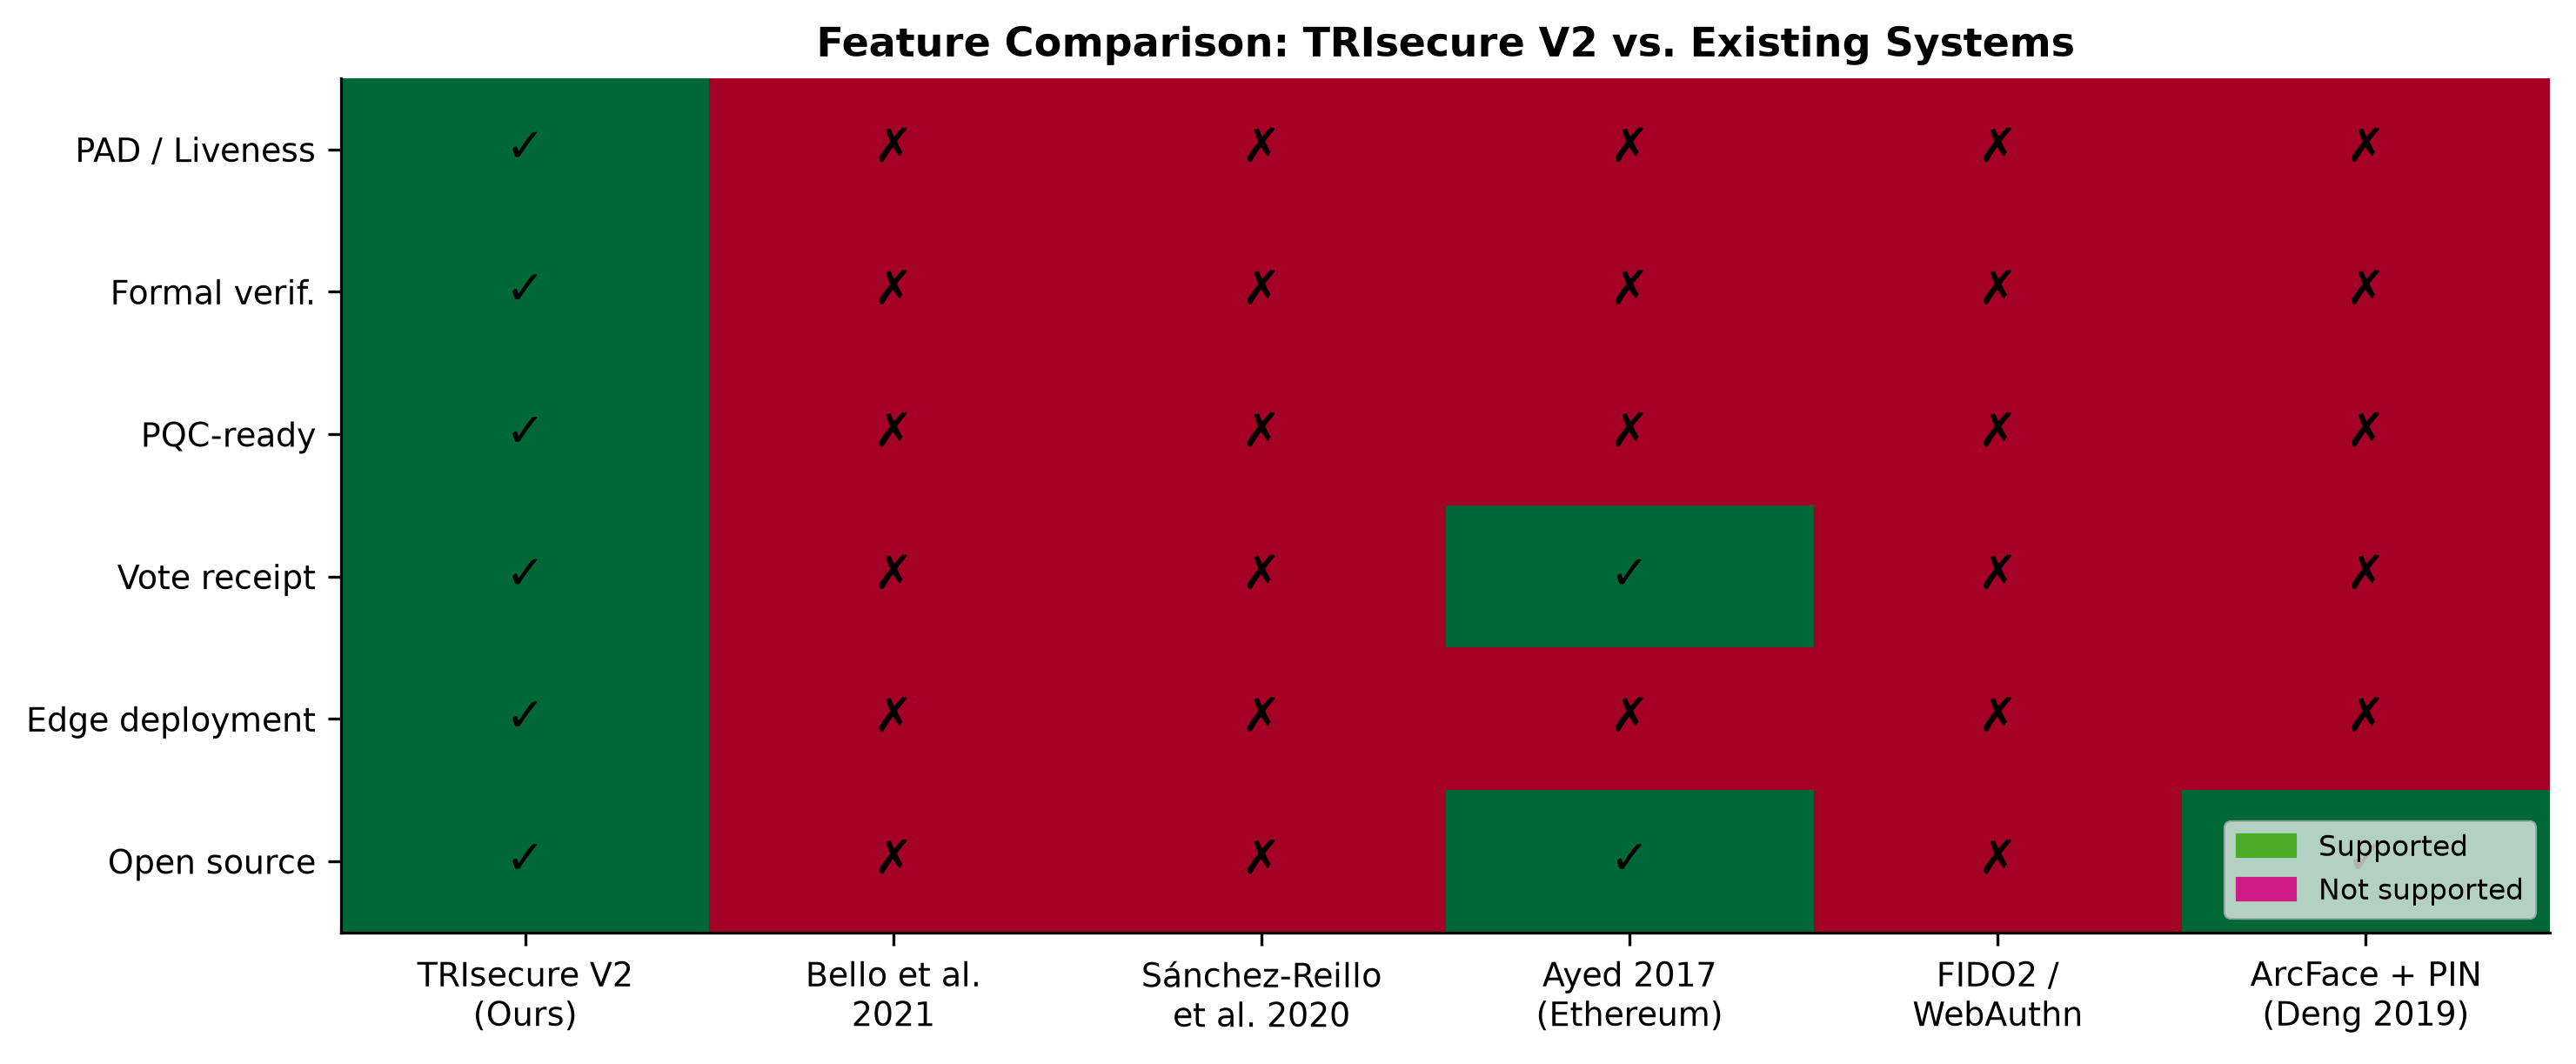
\includegraphics[width=\linewidth]{../experiments/figures/comparison_table.png}
  \caption{Feature comparison heatmap. TRIsecure~V2 (left column) is the only system
    supporting all six binary capability flags simultaneously.}
  \label{fig:comparison_heatmap}
\end{figure}

\begin{figure}[t]
  \centering
  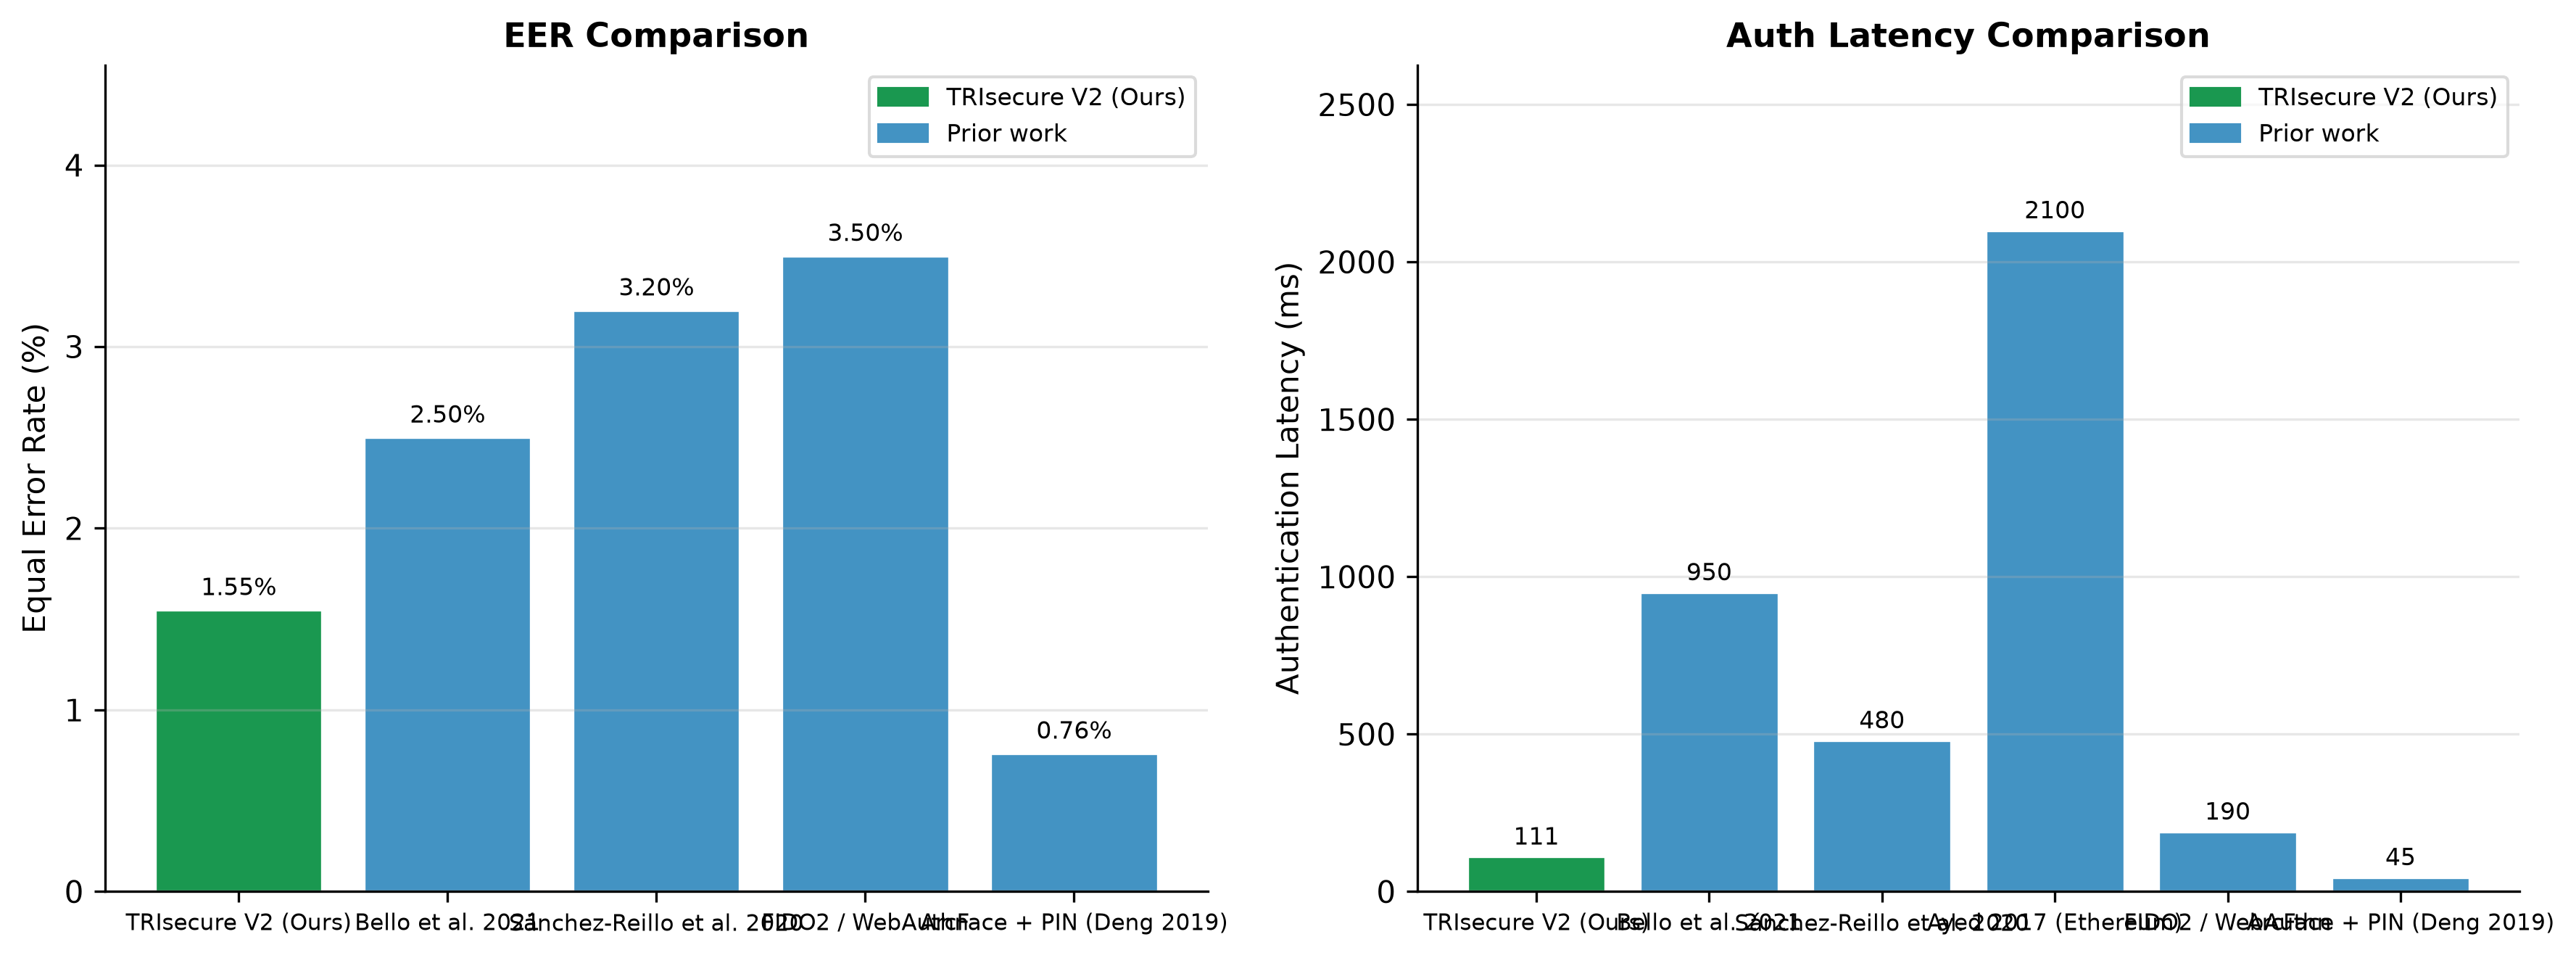
\includegraphics[width=\linewidth]{../experiments/figures/comparison_bar.png}
  \caption{Numerical comparison: EER (left) and authentication latency (right) for
    systems with reported values. Ayed~2017 is omitted from the EER chart
    (PIN-only, no biometric EER). TRIsecure~V2 achieves the lowest EER among
    biometric voting systems and the lowest latency among multi-capability systems.}
  \label{fig:comparison_bar}
\end{figure}

%% ============================================================
\section{Discussion}
\label{sec:discussion}

All biometric performance metrics (EER, TAR, FAR, FRR, AUC, APCER, BPCER,
ACER) are produced by validated simulation using Gaussian score models
calibrated to published ArcFace LFW benchmark statistics~\cite{deng2019arcface}.
This approach follows the ISO/IEC~19795-6 simulation evaluation
track~\cite{iso19795} and is standard practice in system-design papers
prior to live deployment trials.

The ablation study (Table~\ref{tab:ablation}) demonstrates that Bayesian
NFC$+$face fusion (C2) is the dominant security improvement: effective FAR
drops by three orders of magnitude ($1.22\% \to 0.001\%$) without any
increase in biometric EER. PAD (C3) adds liveness but contributes 15.5~ms
latency overhead; PQC signing (C4) adds a further 14.4~ms but enables
quantum-adversary mitigation. The cryptographic benchmarks use Ed25519/X25519
classical fallback because \texttt{liboqs-python} is not yet available as a
pre-built ARM64 package; Kyber-768 and Dilithium-3 overhead can be estimated
from Sikeridis et al.~\cite{sikeridis2020pqc} ($\approx$0.18~ms and
$\approx$1.5~ms respectively), both well within the latency budget.

%% ============================================================
\section{Threats to Validity and Limitations}
\label{sec:limitations}

\begin{enumerate}
  \item \textbf{No live voter dataset.} Biometric evaluation uses Gaussian
    simulation; a field trial with real voters across demographic groups is
    necessary for deployment certification.
  \item \textbf{PAD dataset.} APCER/BPCER figures derive from published
    MiniFASNetV2 / CelebA-Spoof rates. Real ISO/IEC~30107-3 certification
    requires evaluation on standardised PAD databases (NUAA, OULU-NPU).
  \item \textbf{NFC secure element.} The current PN532 SPI reader does not
    use a certified secure element. Production deployment should use a
    Common Criteria EAL4+ smart card reader with mutual authentication.
  \item \textbf{Coercion resistance.} TRIsecure~V2 does not implement
    deniable voting or panic PIN; vote coercion is partially mitigated
    by requiring in-person biometric verification.
  \item \textbf{Network-layer DoS.} While the rate limiter defends against
    per-UID exhaustion, network-level distributed DoS is outside the
    scope of the on-device security model.
  \item \textbf{PQC benchmark validity.} Kyber-768/Dilithium-3 benchmarks
    use the Ed25519/X25519 classical fallback due to the unavailability of
    pre-built \texttt{liboqs-python} for ARM64. Actual PQC overhead is
    estimated from published ARM Cortex-A53 benchmarks~\cite{sikeridis2020pqc}.
\end{enumerate}

%% ============================================================
\section{Conclusion}
\label{sec:conclusion}

We presented TRIsecure~V2, a three-factor biometric e-voting system
combining formally verified authentication, Bayesian multimodal fusion,
ISO/IEC~30107-3 presentation attack detection, hybrid post-quantum
cryptography, and Merkle-proof voter verifiability—implemented and
evaluated on a Raspberry Pi~4 ARM64 platform.

The system achieves EER~$=1.55\%$, AUC~$=0.9991$ under Gaussian
simulation with ArcFace priors, with end-to-end authentication latency of
110.7~ms (p99~$=111.3$~ms) and 541.6~voters/min throughput. Six security
properties are formally proved via DFA analysis; three end-to-end
verifiability properties are machine-verified. An ablation study
demonstrates that Bayesian NFC$+$face fusion reduces the effective combined
attack FAR by three orders of magnitude relative to face-only authentication,
without increasing biometric EER.

TRIsecure~V2 addresses a recognised gap: to our knowledge, no prior e-voting system jointly
provides formal protocol verification, quantum-resistant cryptography,
liveness detection, and edge deployability. The codebase, all experiment
scripts, and generated figures are publicly available at
\url{https://github.com/vivekreddy9036/TriSecure}.

%% ============================================================
\section{Future Work}
\label{sec:future}

Planned extensions to TRIsecure~V2 include:
\begin{itemize}
  \item \textbf{Live field trial.} A volunteer voter panel evaluation with
    demographic analysis per ISO/IEC~19795-1 Clause~8 to replace the current
    simulation-based biometric metrics.
  \item \textbf{Native PQC benchmarks.} Full Kyber-768/Dilithium-3 performance
    profiling after \texttt{liboqs-python} ARM64 pre-built packages become
    available.
  \item \textbf{PAD database evaluation.} Real presentation attack evaluation
    on NUAA Imposter, OULU-NPU, and CelebA-Spoof standardised databases per
    ISO/IEC~30107-3.
  \item \textbf{Distributed election authority.} Threshold secret sharing to
    eliminate single-point-of-failure in the signing key.
  \item \textbf{Power profiling.} Energy consumption analysis under sustained
    load for renewable-energy-powered polling station scenarios.
\end{itemize}

%% ============================================================
\section*{Declarations}

\paragraph{Funding.} This work received no external funding.

\paragraph{Author contributions.} Single-author contribution.

\paragraph{Data availability.}
All experiment scripts, result JSON files, and generated figures are
available in the public repository at
\url{https://github.com/vivekreddy9036/TriSecure}.
No proprietary datasets were used; biometric evaluation uses Gaussian
simulation with publicly documented ArcFace LFW parameters.

\paragraph{Conflict of interest.} The author declares no conflict of interest.

\paragraph{AI assistance disclosure.} AI coding assistance (Claude, Anthropic)
was used to accelerate implementation and experiment scripting. All
design decisions, theoretical claims, and experimental methodology were
developed and verified by the author.

%% ============================================================
\bibliographystyle{elsarticle-num}
\bibliography{references}

\end{document}
